% Template used by paper.py; paper.tex is generated from it.
\documentclass[conference]{IEEEtran}
\IEEEoverridecommandlockouts
\usepackage[utf8]{inputenc}
\usepackage[T1]{fontenc}
\usepackage{cite}
\usepackage{amsmath,amssymb}
\usepackage{graphicx}
\usepackage{booktabs}
\usepackage{url}
\usepackage[hidelinks]{hyperref}
\usepackage{microtype}

\begin{document}

\title{Seven Daily Profiles, Three, or None?\\ Weekday, Day Type and Weather in the Daily Load Shape of U.S. Balancing Authorities\\
\large Cardinal Grid Notes, No.\ 2 \quad <<doi_line>>}

\author{\IEEEauthorblockN{Ricardo W. C. Guerra Filho}
\IEEEauthorblockA{Cardinal Grid (independent open initiative)\\
ORCID 0000-0001-6699-9951 \quad ricardo.guerra@cardinalgrid.com}}

\maketitle

\begin{abstract}
Anomaly detection, gap repair and short-term forecasting of electricity load all rely on a notion of the typical daily profile, and practice differs on how many profiles to keep: one per weekday, or one per day type (workday, Saturday, Sunday), each with a list of special days. This note compares the two, and several alternatives, on the public EIA-930 record of <<n_bas>> U.S. balancing authorities (BAs) from <<first_prose>> to <<last_prose>> (<<ba_days>> BA-days). The daily shape is defined as the 24 hourly demand values divided by the daily mean, in local time; profiles are causal medians over a reference set of earlier days, and models differ only in how that set is chosen. Seven weekday profiles have a higher out-of-sample shape error than three day-type profiles in every BA (mean relative loss <<g7_loss>>), because mid-week profiles differ by <<idx_tue_wed>> units of day-to-day noise while the reference set shrinks fivefold. The length of the reference window matters more than any calendar split: error rises monotonically from <<g3_w2>> at two weeks to <<g3_w16>> at sixteen. Fixed seasonal classes are <<s4_loss>> worse than two recent weeks, whereas adding the same three calendar weeks of the previous year to the recent two reduces error by <<r2a1_gain>> (confidence interval above zero in <<r2a1_up>> BAs). A heating/cooling regime, read from the hour of the daily peak, reduces error by <<regime_oracle>> when known and by <<regime_prev>> when proxied by the previous day, and the days on which the most BAs depart from their profiles are regime transitions rather than holidays. Thanksgiving, Christmas and the two eves resemble Saturdays; Memorial Day, Labor Day and Independence Day resemble Sundays; four minor federal holidays are not distinguishable from ordinary weekdays. Code and results are open.
\end{abstract}

\begin{IEEEkeywords}
load profiles, load forecasting, calendar effects, holidays, balancing authority, EIA-930, anomaly detection
\end{IEEEkeywords}

\section{Introduction}
Most methods that operate on an hourly load series carry, explicitly or not, a model of the typical day. Short-term load forecasting uses calendar variables that distinguish weekdays and holidays \cite{hong2016review,taylor2003double}; anomaly detectors compare each reading with what a normal day would show; gap-filling routines borrow the shape of equivalent days. Practice differs on how fine the calendar should be. One tradition keeps a profile for each of the seven weekdays; another keeps three, for workdays, Saturdays and Sundays; both add a list of special days that follow no profile. The choice is rarely justified with data, and it has consequences: a finer calendar needs more history to estimate each profile, and more history means older data in a series whose shape drifts with the season.

Since July 2015, Form EIA-930 has made the hourly demand of every balancing authority (BA) in the contiguous United States public \cite{eia930monitor}, so the question can be settled empirically and at once for the whole interconnected system. This note does that. It asks three things: whether seven profiles beat three out of sample; how long the reference history should be and whether the season should enter as a class or as an analog; and which days are actually special, both from a fixed list and from the data. The purpose is descriptive and the recommendations are conditional on the evidence presented.

\section{Data}
\subsection{Source and preparation}
Hourly demand (``hourly integrated values in megawatts by hour ending time'' \cite{eia930instructions}) was taken from EIA's six-month balance files for <<first_prose>> to <<last_prose>> \cite{eia930monitor}, in each BA's local time as reported in the files. A BA-day is valid when at least 23 of its 24 hours have positive demand; on the two daylight-saving transition days per year the missing hour is interpolated and the duplicated hour averaged. Days in which any hour falls below 20\% or above 300\% of the daily mean are removed as corrupted (<<dropped>> days). A BA enters the study with at least 600 valid days and a mean demand of at least 500~MW; <<n_bas>> of <<n_files>> BAs in the files qualify, giving <<ba_days>> BA-days. EIA's imputed values are used as reported.

\subsection{Daily shape}
The shape of BA-day $d$ is the vector $s_d \in \mathbb{R}^{24}$ with $s_{d,h} = D_{d,h} / \bar{D}_d$, where $D_{d,h}$ is demand in hour ending $h$ and $\bar{D}_d$ the daily mean. Dividing by the mean separates the shape of the day from its level; the level, which depends on weather and season in ways well studied elsewhere \cite{hyndman2010density}, is not analysed here.

\subsection{Calendar}
Weekday and day type (workday, Saturday, Sunday) are taken from the local date. The a-priori special-day list consists of U.S. federal holidays and their observed days, the day after Thanksgiving, 24 and 31 December, and Super Bowl Sunday; it covers <<special_share>> of BA-days. A \emph{heating/cooling regime} is defined from the load itself: a day is a morning-peak day if its highest hour is 12:00 or earlier, which in practice is an electric-heating morning, and an afternoon/evening-peak day otherwise.

\section{Methods}
\subsection{Causal profile models}
For each day $d$ and each model, the profile $\hat{s}_d$ is the hour-by-hour median of the shapes of a reference set $R_d$ of earlier days. Nothing after $d$ is used, and special days are never references. The models differ only in $R_d$. In the \emph{grouping} family, $R_d$ contains the days of the same group as $d$ in the previous $W$ weeks, where the group is defined by one of five calendars: G1, a single group; G2, week versus weekend; G3, workday, Saturday, Sunday; G5, Monday, Tuesday--Thursday, Friday, Saturday, Sunday; G7, one group per weekday. The window $W$ is 8 weeks for the model comparison and is varied from 2 to 16 weeks for the G1, G3 and G7 calendars. A profile is computed only when $|R_d| \ge 3$ ($\ge 2$ at $W=2$).

Three further models test the season and the weekday signature. A \emph{fixed-season} model (S4) crosses the four meteorological seasons with the three day types and uses the previous 52 weeks. A \emph{seasonal-analog} model uses, as references, the days of the same day type within $\pm 21$ days of the same calendar date one year earlier (A1), or one and two years earlier (A2), either alone or in union with the previous two weeks (R2+A1, R2+A2). A \emph{hybrid} model adds to the recent G3 profile a per-weekday offset, the median over the previous 52 weeks of the residual $s_j - \hat{s}_j$ for days $j$ of the same weekday. Finally, a \emph{regime} model splits G3 by the heating/cooling regime, once with the day's own regime (an oracle that stands for a perfect temperature forecast) and once with the previous day's regime (a causal proxy that needs no external data).

\subsection{Error and tests}
The shape error of day $d$ under a model is the mean absolute percentage error over the 24 hours,
\begin{equation}
e_d = \frac{100}{24}\sum_{h=1}^{24}\frac{|\hat{s}_{d,h} - s_{d,h}|}{s_{d,h}} .
\end{equation}
Models are compared on normal (non-special) days for which every model produces a profile. For each BA, the difference in daily error between two models is summarised by its mean, a 95\% bootstrap confidence interval (2000 resamples of days) and a sign test. A BA is said to \emph{need} the finer model when the interval excludes zero and the relative gain exceeds 5\%; this criterion was fixed before the data were examined.

\subsection{Weekday distinctness}
For each BA, long-run weekday profiles $p_w$ ($w = 1,\dots,7$) are the medians of all normal days of that weekday. The distance between two weekdays is the MAPE between their profiles, and the day-to-day noise is the median over all normal days of the MAPE between a day's shape and its own weekday profile. The ratio of the two is a dimensionless distinctness index: a value below 1 means that the two weekdays differ by less than two days of the same weekday do. Average-linkage hierarchical clustering of the index matrix, cut at 1, gives the number of weekday groups that the data distinguish.

\subsection{Special days}
For each special day and BA-year, the day's shape is compared with three causal profiles from the same 8-week window: that of its own weekday, of Saturday and of Sunday; for special days falling on a weekend only the last two apply. The closest profile is recorded. For Super Bowl Sunday, the residual against the median of the non-special Sundays within five weeks is reported by local hour and by time zone. Data-driven special days are the dates with the highest median shape error under G3 across BAs, restricted to dates on which at least 80\% of BAs report.

\section{Results}
\subsection{Seven profiles against three}
Fig.~\ref{fig:models} shows the mean shape error of the five grouping calendars at $W = 8$, one point per BA, and Table~\ref{tab:models} the means over BAs. G7 has a higher error than G3 in every one of the <<n_bas>> BAs, with the bootstrap interval entirely below zero in <<ci_below>> of them; the mean relative loss is <<g7_loss>>. G5 also loses to G3 (<<g5_loss>>). The distinctness index explains why (Fig.~\ref{fig:distinct}): the median index between Tuesday and Wednesday is <<idx_tue_wed>>, between Monday and Thursday <<idx_mon_thu>>, between Thursday and Friday <<idx_thu_fri>>, whereas between Wednesday and Sunday it is <<idx_wed_sun>>. Cutting the clustering at an index of 1 yields a single weekday group in <<n_one_cluster>> BAs and two groups (workdays; Saturday and Sunday) in <<n_two_clusters>>: <<two_cluster_bas>>. The hybrid model confirms that the weekday signature is real but immaterial: it improves Mondays by <<hyb_mon>> and Fridays by <<hyb_fri>> percentage points, costs the same on the other days, and changes the overall error by <<hyb_gain>> relative.

\begin{figure}[t]
\centering
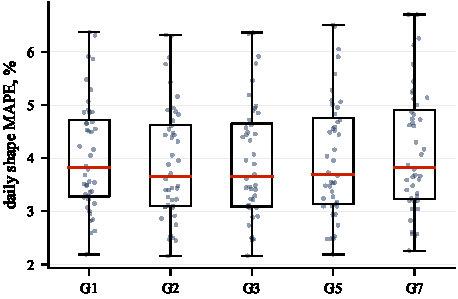
\includegraphics[width=\columnwidth]{figures/fig1_models.pdf}
\caption{Mean out-of-sample daily shape MAPE of the five grouping calendars with an 8-week reference window; one point per BA, boxes over the <<n_bas>> BAs. Source: EIA-930 \cite{eia930monitor}, <<first_month>> to <<last_month>>.}
\label{fig:models}
\end{figure}

\begin{table}[t]
\caption{Mean daily shape MAPE over BAs, normal days, <<first_month>> to <<last_month>>.}
\label{tab:models}
\centering
\begin{tabular}{llr}
\toprule
Model & Reference set (day type $\times$ history) & MAPE \\
\midrule
<<model_rows>>
\bottomrule
\end{tabular}
\end{table}

\begin{figure}[t]
\centering
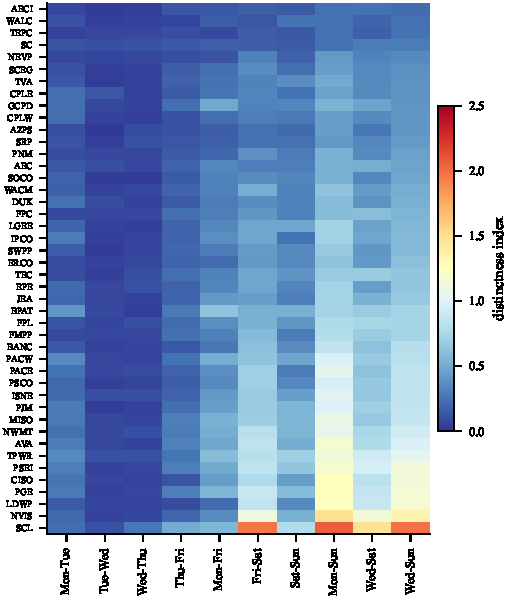
\includegraphics[width=\columnwidth]{figures/fig2_distinctness.pdf}
\caption{Distinctness index between pairs of weekdays, one row per BA, sorted by the Wednesday--Sunday index. An index of 1 means that the two weekday profiles differ as much as two days of the same weekday do.}
\label{fig:distinct}
\end{figure}

\subsection{Reference window and season}
Fig.~\ref{fig:window} shows the error of G1, G3 and G7 against the window length. Error rises monotonically with $W$ for every calendar: G3 goes from <<g3_w2>> at two weeks to <<g3_w16>> at sixteen, and a single profile from the last three weeks (<<g1_w3>>) beats three profiles from the last six (<<g3_w6>>). The best model in the grid is G3 at $W = <<best_weeks>>$ weeks (<<best_mape>>).

The season enters usefully as an analog rather than as a class (Table~\ref{tab:season}). The fixed-season model S4 is <<s4_loss>> worse than two recent weeks, with the interval below zero in <<s4_below>> BAs. The analogs of the previous year alone are as accurate as the last two weeks (<<a1>> against <<g3_w2_seas>> on the same days); their union with the recent two weeks is better than either (<<r2a1>>), a relative gain of <<r2a1_gain>> with the interval above zero in <<r2a1_up>> BAs and above 5\% in <<r2a1_need>>; two years of analogs give <<r2a2_gain>>. The gain is present in every month and largest from March to June (<<gain_spring>> against <<gain_other>> percentage points in the other months). The exceptions are <<analog_worst>>, where the analogs increase error because the daily shape of those systems is changing from one year to the next.

\begin{figure}[t]
\centering
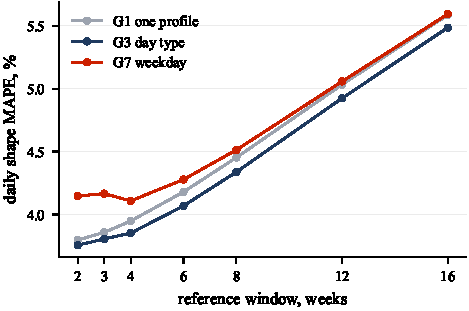
\includegraphics[width=\columnwidth]{figures/fig3_window.pdf}
\caption{Mean daily shape MAPE over BAs against the length of the reference window, for the G1, G3 and G7 calendars.}
\label{fig:window}
\end{figure}

\begin{table}[t]
\caption{Season as a class versus as an analog. Mean daily shape MAPE over BAs on the days where all five models exist; relative gain over the two-week G3 model with the number of BAs whose 95\% interval lies above (or below) zero.}
\label{tab:season}
\centering
\small
\begin{tabular}{llrr}
\toprule
Model & Reference set & MAPE & Gain vs.\ R2 \\
\midrule
<<season_rows>>
\bottomrule
\end{tabular}
\end{table}

\subsection{Heating/cooling regime}
Fig.~\ref{fig:regime} shows, on the left, the monthly share of morning-peak days for five BAs, and on the right the gain of the regime-split G3 model over G3 by BA. In the Southeast and the Northwest more than 40\% of December and January days peak in the morning; in California, New York and New England almost none do. Splitting by the day's own regime reduces the shape error by <<regime_oracle>> on average, by more than 5\% in <<regime_oracle_n>> BAs and by up to <<regime_top_gain>> in <<regime_top_ba>>; the previous-day proxy gives <<regime_prev>> on average and more than 5\% in <<regime_prev_n>> BAs. The dates on which the most BAs depart from their profiles at once (Table~\ref{tab:dates}) are regime transitions, the first cold morning of autumn and the first hot afternoon of spring, rather than holidays; the highest-ranked holiday, Thanksgiving, appears at rank <<tg_rank>>.

\begin{figure*}[t]
\centering
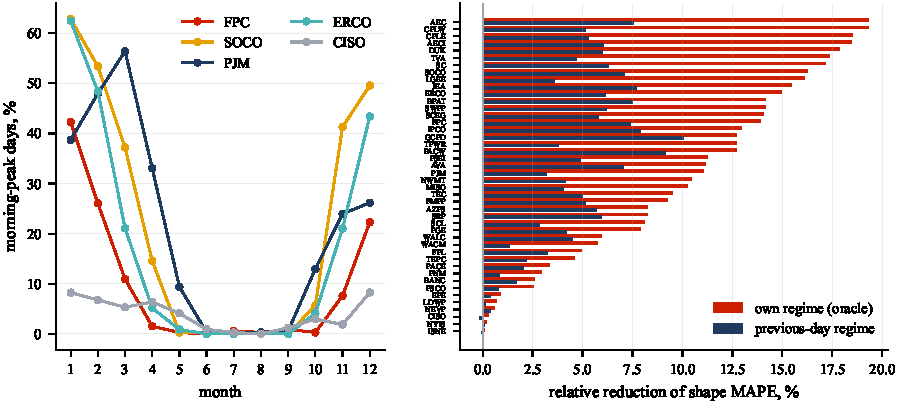
\includegraphics[width=\textwidth]{figures/fig4_regime.pdf}
\caption{Left: share of days whose peak falls at hour ending 12 or earlier, by month, for five BAs. Right: relative reduction of shape MAPE from splitting the three day types by the heating/cooling regime, using the day's own regime (oracle) and the previous day's regime (causal), by BA.}
\label{fig:regime}
\end{figure*}

\begin{table}[t]
\caption{Dates with the largest median shape error across BAs (G3, 8 weeks), among dates on which at least 80\% of BAs report.}
\label{tab:dates}
\centering
\small
\begin{tabular}{llrr}
\toprule
Date & Weekday & Median MAPE & Special day \\
\midrule
<<date_rows>>
\bottomrule
\end{tabular}
\end{table}

\subsection{Special days}
Table~\ref{tab:holidays} gives, for each special day, the median error against the three candidate profiles and the profile most often closest. Three groups appear. Thanksgiving, Christmas Day, Christmas Eve and New Year's Eve are closest to Saturday in a majority of BA-years; Memorial Day, Labor Day and Independence Day are closest to Sunday; MLK Day, Presidents' Day, Columbus Day and Veterans Day are closest to their own weekday, i.e.\ they are not special days for load. Juneteenth, observed federally only since 2021, is split. Super Bowl Sunday shows a residual of $-3$ to $-4$\% of the daily mean during the game, shifted by time zone (Fig.~\ref{fig:superbowl}), and is closer to a Saturday than to a Sunday in <<sb_sat_share>> of BA-years.

\begin{table}[t]
\caption{Special days: median shape MAPE against the profile of the day's own weekday, of Saturday and of Sunday (8-week window), and the profile most often closest, with its share of BA-years.}
\label{tab:holidays}
\centering
\small
\begin{tabular}{lrrrrl}
\toprule
Day & $n$ & Own & Sat. & Sun. & Closest \\
\midrule
<<holiday_rows>>
\bottomrule
\end{tabular}
\end{table}

\begin{figure}[t]
\centering
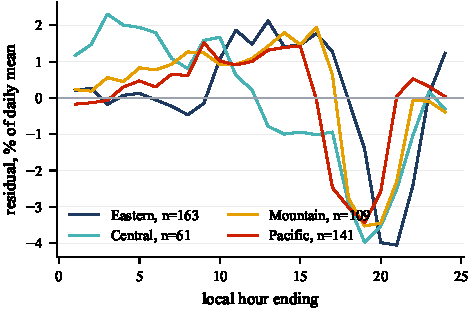
\includegraphics[width=\columnwidth]{figures/fig5_superbowl.pdf}
\caption{Super Bowl Sunday: median shape residual against neighbouring Sundays, by local hour and time zone; $n$ is the number of BA-years.}
\label{fig:superbowl}
\end{figure}

\begin{figure}[t]
\centering
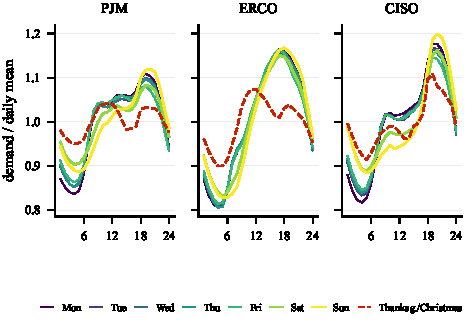
\includegraphics[width=\columnwidth]{figures/fig6_examples.pdf}
\caption{Long-run weekday profiles of three BAs (medians over all normal days) with the median Thanksgiving and Christmas Day shape overlaid.}
\label{fig:examples}
\end{figure}

\section{Discussion}
\subsection{Interpretation}
The results separate three effects that are usually bundled under ``calendar''. The weekend effect is real in every BA and dominant in the urban and West-Coast systems. The weekday effect within the working week exists, is stable, and is smaller than the day-to-day noise; estimating it costs more history than it returns, whether by grouping or by a long-run offset. The seasonal effect is the largest of the three and is best handled by recency, with the previous year's analog as a complement that anticipates where the shape is going, and worst handled by fixed classes. Above all three sits the weather regime: on the days that matter most for operations, when the peak moves from the evening to the morning, no calendar model is informed, and a temperature-conditioned day type recovers a large part of the error. That the largest coordinated departures from the typical shape are regime transitions rather than holidays is, for anomaly detection, the central finding: a detector that compares readings with a calendar profile will raise its loudest alarms on the first cold morning of the year.

\subsection{Recommendations}
For profile-based methods on U.S. BA load the evidence supports: (i) three day types rather than seven; (ii) a reference set of the last two weeks plus the same three calendar weeks of the previous year, with the analog dropped where the shape is known to be changing year over year; (iii) a special-day list restricted to New Year's Day, Memorial Day, Independence Day, Labor Day, Thanksgiving and the day after, Christmas Eve and Day, New Year's Eve and Super Bowl Sunday, each mapped to the Saturday or Sunday profile as in Table~\ref{tab:holidays}; and (iv) a heating/cooling regime as an additional day type wherever a BA shows winter morning peaks, driven by a temperature forecast when available and by the previous day's regime otherwise.

\subsection{Limitations}
Only the shape is analysed; a day whose level changes without a change of shape is invisible here. The regime is read from the load rather than from temperature, so the oracle split is an upper bound and the previous-day split a lower bound for a temperature-driven model. The 8-week window of the model comparison is not the best window, but the ranking of calendars does not change with the window. BAs spanning several time zones report in one and their profiles are blends. The special-day list is national; state holidays and local events are not represented. Results are for aggregate BA load and need not hold at the feeder or substation level, where the weekday signature can be larger.

\section{Conclusion}
On the public record of <<n_bas>> U.S. balancing authorities, three day-type profiles estimated from recent days outperform seven weekday profiles everywhere, the length and recency of the reference history matter more than the calendar, the previous year's analog days add to recent days, and the heating/cooling regime moves the daily shape more than any holiday. A short list of special days, mapped to Saturday or Sunday profiles, covers the calendar exceptions that the data support. These choices are being adopted in the open anomaly-detection tool of the same initiative, and a subsequent note will replace the load-derived regime with a temperature-driven one.

\section*{Data and Code Availability}
Data: EIA-930 six-month balance files \cite{eia930monitor}, prepared with \cite{guerra2026scorecard}. This note, its figures and tables are reproduced by \texttt{analysis.py} and \texttt{paper.py} in \url{https://github.com/cardinalgrid/notes} (code Apache-2.0, text and figures CC BY 4.0).

\bibliographystyle{IEEEtran}
\bibliography{references}

\end{document}
